% Niveau :      PCSI
% Discipline :  Mécaflu
%Mots clés :    

\begin{exercise}{Le barrage de Cap de Long}{1}{Sup, Spé}
{Statique des fluides, Mécanique, Moment cinétique}{bermu}

\begin{questions}
    \questioncours Redémontrer l'équation de la statique des fluides et donner l'expression de la pression dans une retenue d'eau en fonction de la profondeur $z$. 
\begin{EnvUplevel}
Dans ce qui va suivre, on s'intéresse à comment construire un barrage tout en évitant la catastrophe. Il existe deux grands types de barrages, les barrages poids et les barrages voûte :
\begin{figure}[H]
    \centering
    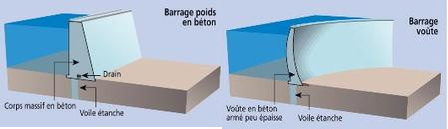
\includegraphics[width=\linewidth]{mecaflu/statiqueflu/capdelong1.png}
    \vspace{-2em}
    \caption{Les deux familles de barrages : barrage poids et barrage voûte.}
\end{figure}
\end{EnvUplevel}
    \question Commençons par étudier un barrage poids, de hauteur $H$, et d'épaisseur au sol $\ell$.
\begin{parts}
    \part Justifier qualitativement la forme du barrage.
    \part Modéliser la force totale qui s'applique sur la paroi du barrage (on prêtera attention au traitement de la pression atmosphérique). \\
    Application numérique, à mettre en perspective avec des ordres de grandeur connus. \label{que:forcetot}
    \part Exprimer la condition d'équilibre du barrage et donner une condition sur l'épaisseur maximale au sol et la hauteur.
    \part Évaluer la force exercée par le sol sur le barrage nécessaire pour que celui-ci ne soit pas emporté. Mettre ce résultat en perspective avec celui de la question \ref{que:forcetot}
\end{parts}

    \question Continuons avec un barrage voûte, de hauteur $H$, de rayon de courbure $R_\textsc{c}$ et d'épaisseur $\ell$.
\begin{parts}
    \part Quelle est qualitativement la différence avec la configuration précédente. Quels avantages ou inconvénients ?
    \part La force totale qui s'applique sur la paroi du barrage est-elle sensible à la géométrie du barrage ?
    \part Évaluer la force exercée par le sol \underline{et les contreforts} sur le barrage nécessaire pour que celui-ci ne soit pas emporté. Comparer avec les résultats de la question précédente.
\end{parts}
\end{questions}

\begin{wrapfigure}{l}{0.55\textwidth}
    \centering
    \vspace{-1em}
    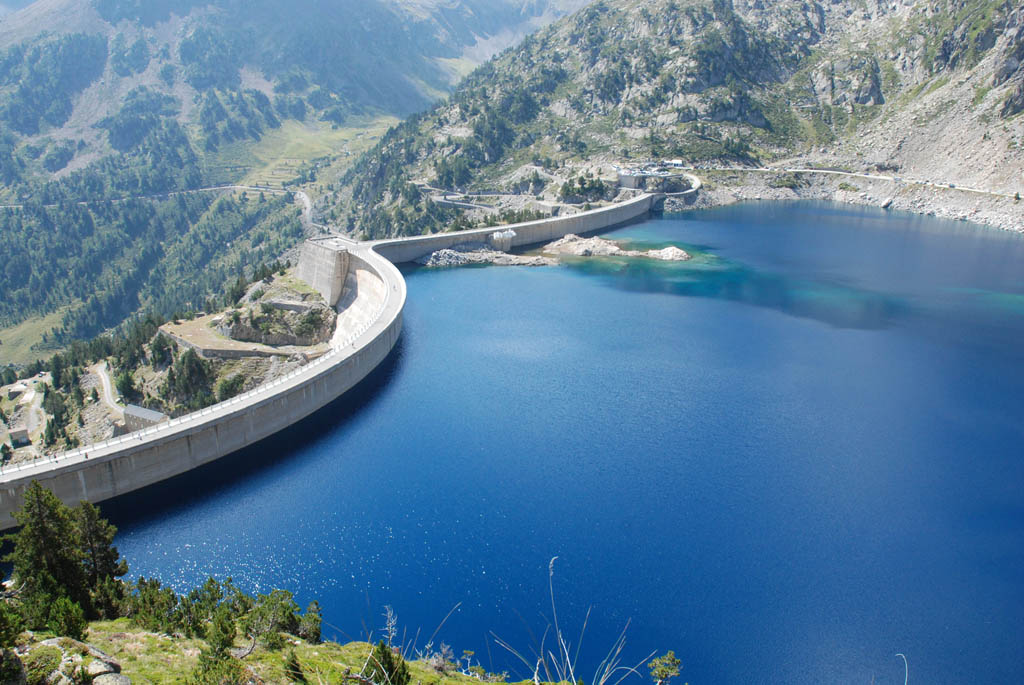
\includegraphics[width=0.8\linewidth]{mecaflu/statiqueflu/capdelong2.png}
    \vspace{-1em}
    \caption{Le barrage de Cap de Long, 101 m de haut, est la plus grande retenue d'eau des Pyrénées.}
\end{wrapfigure}


\paragraph{Données :}
\begin{itemize}
    \item pesanteur terrestre $g = 10$ m$^2\cdot$s$^{-1}$,
    \item densité du béton armé $d= 3,5$.
\end{itemize}
\end{exercise}